\begin{figure}
  \centering
    \begin{tikzpicture}
      \node[inner sep=0pt] (img) at (-8.25,3cm)
           {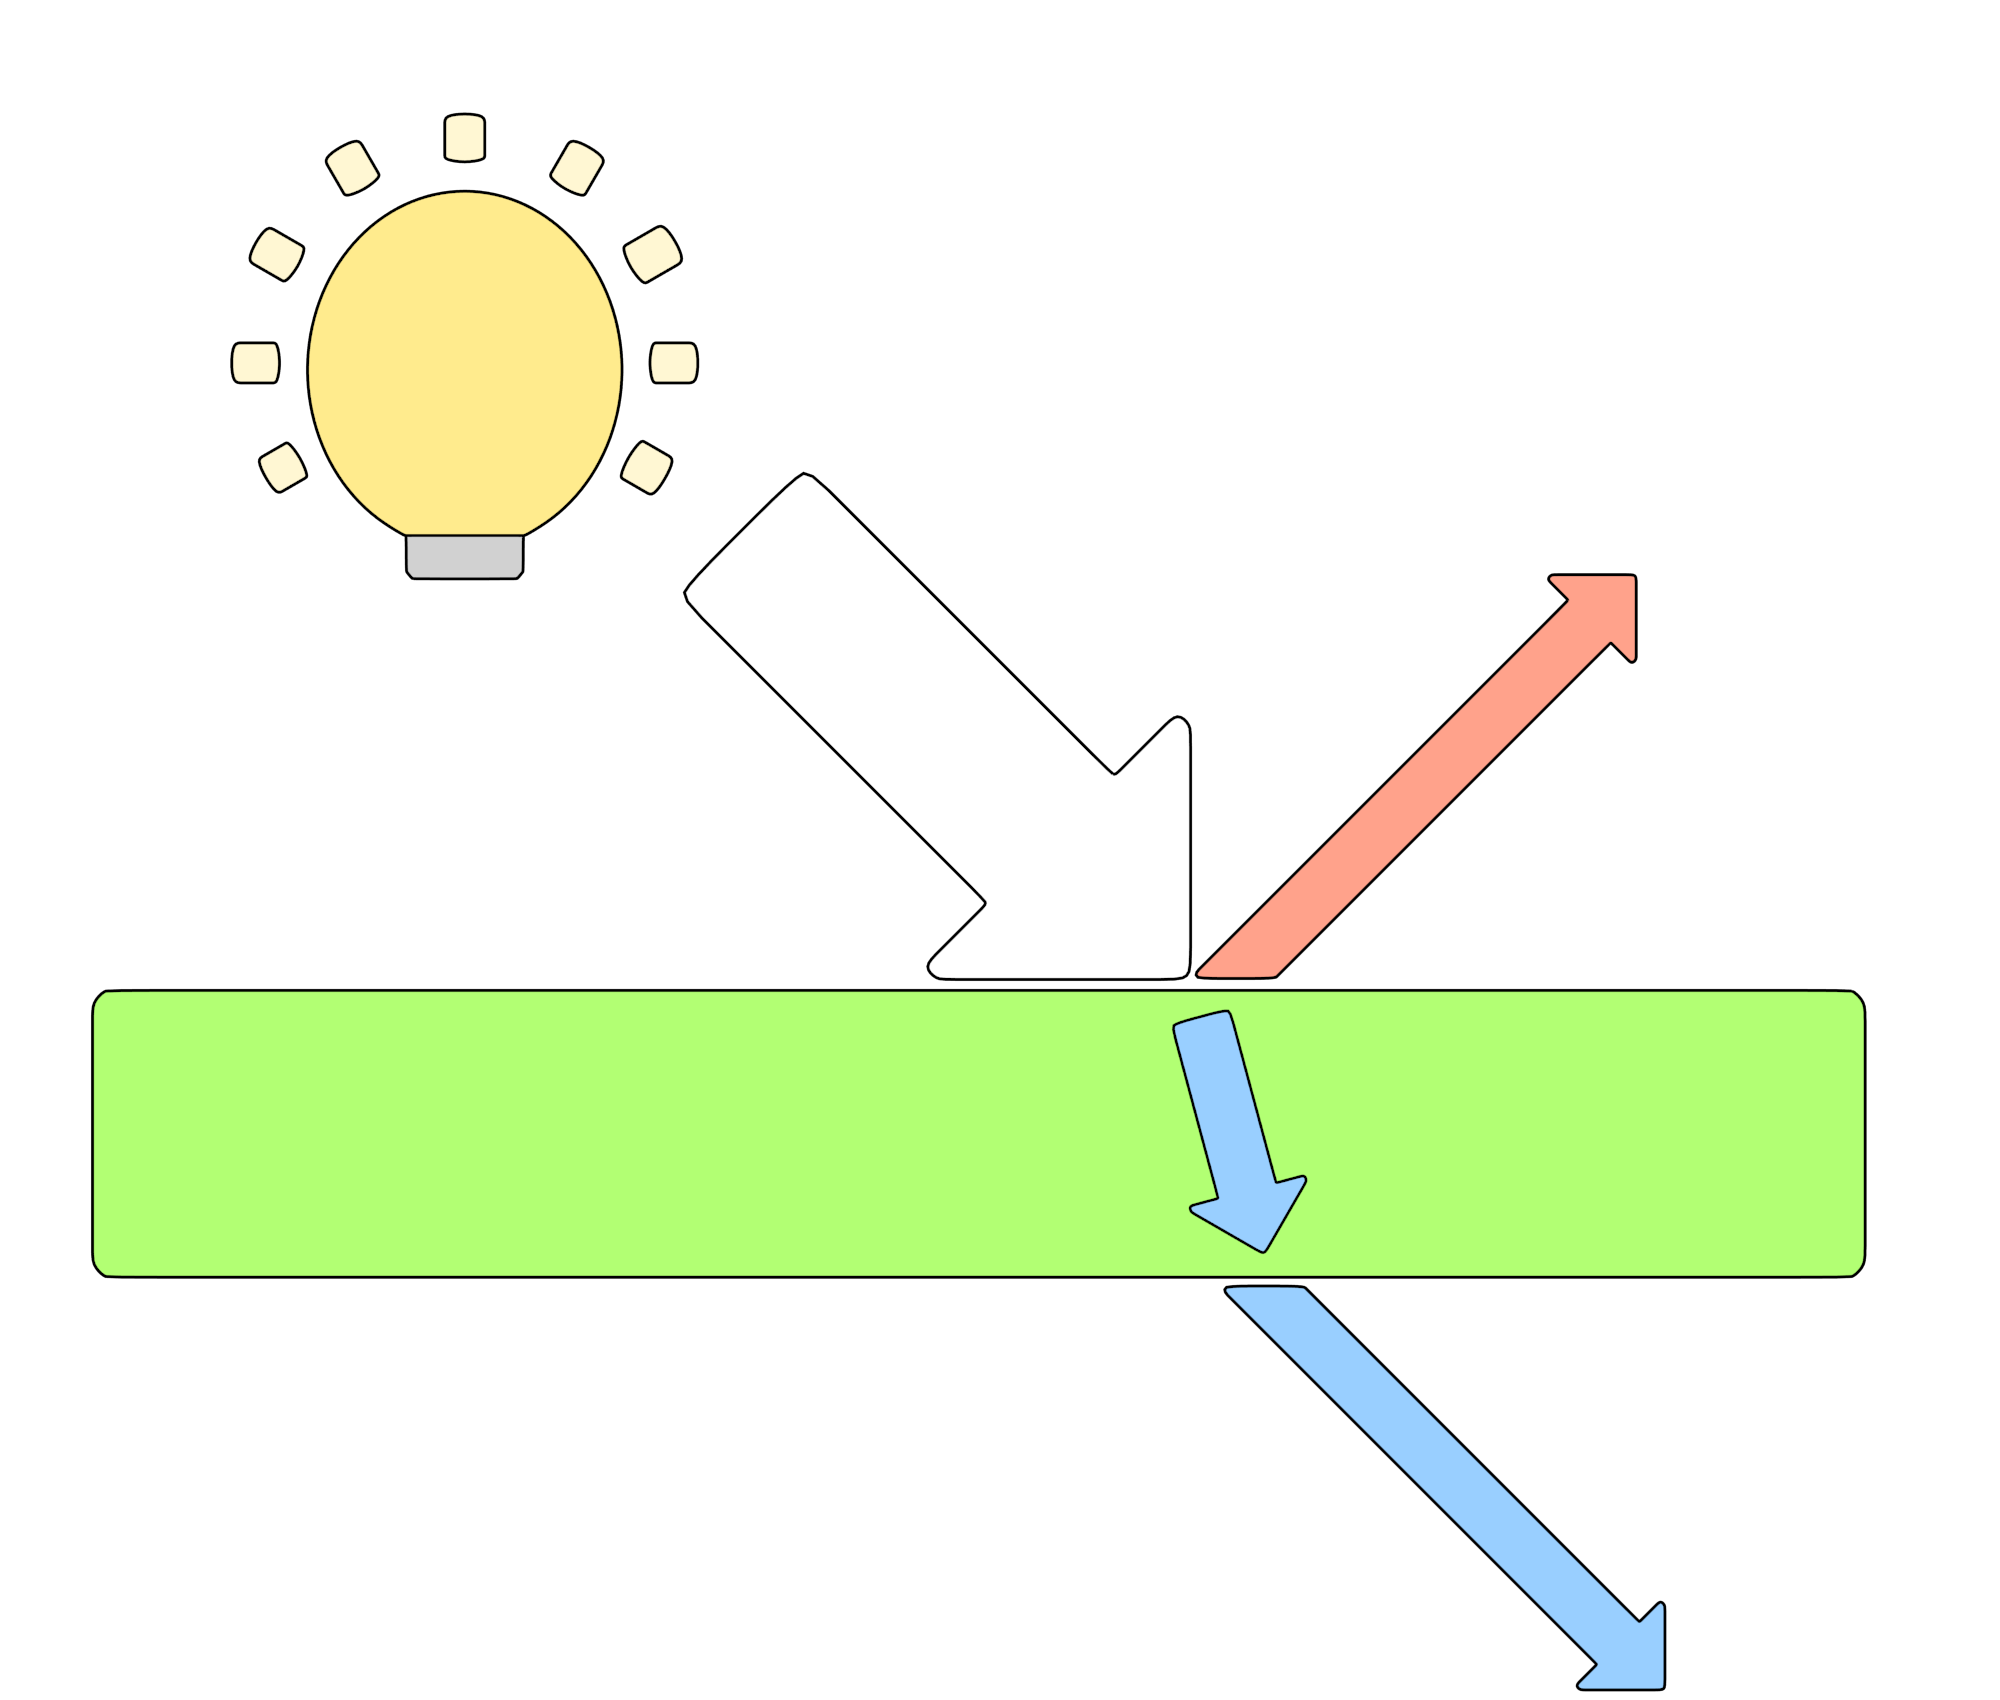
\includegraphics[width=0.65\textwidth]{./img/raw/fw-licht-rgba.png}};

           \node (l1) at (-11, 1.65) {Absorptie};
           \node (l2) at (-7.55, 0.0) {Transmissie};
           \node (l3) at (-5.25, 3) {Reflectie};
           \node (l3) at (-8.5, 5.25) {Lichtbron};
           \node (l4) at (-9.8, 3) {Lichtstraal};
    \end{tikzpicture}
  \caption{Absorptie, reflectie en transmissie van licht.}
  \label{fig:fw-licht}
\end{figure}
